\section{Task 6: From Light Blond to Black}
\label{sec:task6}

\subsection{Results for All Beer Colours}
\label{sec:task6-results}
The full quality-constrained model from Task 5 is solved for each colour class. Black beer is modelled as $\EBC \geq 120+\epsilon_{\EBC}$, with $\epsilon_{\EBC}=10^{-6}$, because the assignment specifies $\EBC>120$.

\begin{table*}[!t]
\renewcommand{\arraystretch}{1.15}
\caption{Task 6 Results for All Beer Colours}
\label{tab:task36-colors}
\centering
\small
\begin{tabular}{@{}llrlrp{0.24\textwidth}@{}}
\toprule
Colour & EBC range & Feasible & Cost & Achieved EBC & Notes \\
\midrule
light blond & 6--8 & no & -- & -- & No feasible quality-constrained mix found. \\
blond & 9--12 & yes & 4919.601 & 12.000 & Uses the upper blond boundary. \\
gold & 13--19 & yes & 4883.000 & 14.535 & Cheapest feasible colour in this run. \\
amber & 20--29 & yes & 4891.923 & 20.000 & Same setup as Task 5. \\
copper & 30--45 & yes & 4908.251 & 30.000 & Uses the lower colour boundary. \\
brown & 46--75 & yes & 4934.376 & 46.000 & Darker colour requires a different source mix. \\
dark brown & 76--120 & yes & 4983.359 & 76.000 & Upper bound remains 120. \\
black & $>120$ & yes & 5061.830 & 120.000001 & Modelled as $120+\epsilon_{\EBC}$. \\
\bottomrule
\end{tabular}
\end{table*}

\subsection{Cost as a Function of Beer Colour}
\label{sec:task6-plot}
The minimum cost for each feasible colour is plotted in Figure~\ref{fig:task36-cost-color}.

\begin{figure}[!t]
\centering
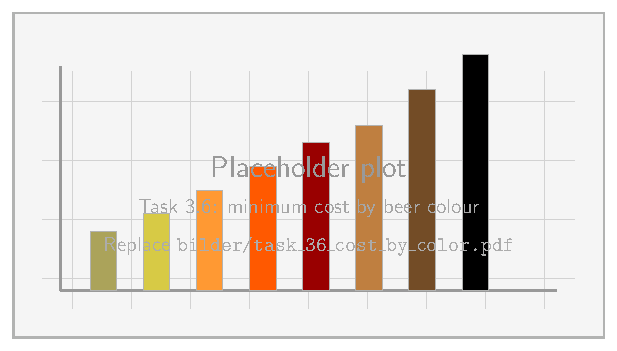
\includegraphics[width=\linewidth]{bilder/task_36_cost_by_color}
\caption{Task 6 minimum cost by beer colour. Replace this placeholder with the plot exported from \texttt{task\_36.ipynb}.}
\label{fig:task36-cost-color}
\end{figure}

\subsection{Explanation}
\label{sec:task6-explanation}
The cost differences are caused by the available EBC values and quality scores in the dataset. Some colours can be reached with cheap ingredients while still satisfying the quality constraints. Other colours require a more expensive mix to move the weighted EBC average into the required interval. In this run, all feasible colour classes use mashing and avoid malting, so the main variation comes from the selected malt and extract sources rather than from different fixed process choices. Light blond is infeasible under the quality-constrained setup, while black is feasible only above the strict 120 EBC boundary represented by $120+\epsilon_{\EBC}$.

% Values in this section come from the updated task_36.ipynb after the black EBC epsilon fix.
